\subsection{Nonlinear Optimization problem}
The objective is to minimize the following cost function:
\begin{align}
\mbox{(B)} : \ \ V(x) = - \frac{\sqrt{(x_1^2 +1)(2x_2^2 + 1)}}{x_1^2 + x_2^2 + 0.5}; \ \  x \in \mathbb{R}^2 \nonumber \\
\end{align}
This is an unconstrained nonlinear optimization problem of the form:
\begin{align}
    V(x) = f(x)
\end{align}
where 
\begin{align}
    V \in \mathbb{R}
\end{align}
This can be solved using search algorithms: 
\begin{itemize}
    \item Steepest descent algorithms 
    \item Secant algorithms
    \item Conjugate gradient method 
\end{itemize}
\subsubsection{Solutions to unconstrained nonlinear problem using our python programs and matlab benchmark \textit{fminunc} function: }
All four algorithms converged to very close local minimal solutions for $x$ with a tolerance set to $tol =1e-8$ and the same initial value of the column vector of $[-1,1]^{T}$ as confirmed in the contour plot in figure 3. The gradient loss of the secant, conjugate and steepest descent algorithm of our Python-implemented sub-programs converged to a minimum at close to 6 iterations while the matlab implementation used the quasi newton method approached the minimum at 5 iterations.
The contour plot of the function $V(x)$ and the minimum solutions of $x$ derived from the 4 algorithms showed that the lowest value of the objective function for the 4 algorithms exists close to the local minima of the function.
\begin{table}[htbp]
\centering
\begin{center}
\begin{tabular}{|c|c|c|c|c|}
\hline
 & \textbf{Steepest Descent} & \textbf{Secant} &\textbf{Conjugate Method} &\textbf{\textit{Matlab}}\\
\hline
Iterations & 6 & 7 &7& 5 \\
\hline
$x$ & 
\begin{bmatrix}
-4.2345e-09 \\
-5.3553e-09 \\
\end{bmatrix}
&\begin{bmatrix}
 -2.8775e-09 \\
 -2.8274e-09 \\
\end{bmatrix} & \begin{bmatrix}
 -1.0739e-04 \\
 -6.8937e-05 \\
\end{bmatrix} &\begin{bmatrix}
   8.8494e-09 \\
    -2.6837e-10 \\  
\end{bmatrix} \\
\hline 
\end{tabular}
\label{table:results}
\caption{Algorithm Performance}
\end{center}
\end{table}

\begin{figure}[h!]
\centering
\begin{subfigure}[t]{0.4\textwidth}
\centering
    \includegraphics[width=\textwidth]{images/python/sd-pB.eps}
\caption{}
\label{fig:Class distribution}
\end{subfigure}
\hfill 
\begin{subfigure}[t]{0.4\textwidth}
\centering
    \includegraphics[width=\textwidth]{images/python/sec-pB.eps}
    \caption{}
    \label{fig:TSNE}
\end{subfigure}
\hfill
\begin{subfigure}[t]{0.4\textwidth}
\centering
    \includegraphics[width=\textwidth]{images/python/cg-pB.eps}
    \caption{}
    \label{fig:TSNE}
\end{subfigure}
\hfill
\begin{subfigure}[t]{0.4\textwidth}
\centering
    \includegraphics[width=\textwidth]{images/matlab/1b_loss.eps}
    \caption{}
    \label{fig:TSNE}
\end{subfigure}
\caption{(a): Steepest descent, (b): Secant method, (c): Conjugate gradient, (d): Matlab: \textit{fminunc - quasi-newton method}}
\end{figure}
\begin{figure}
    \centering
    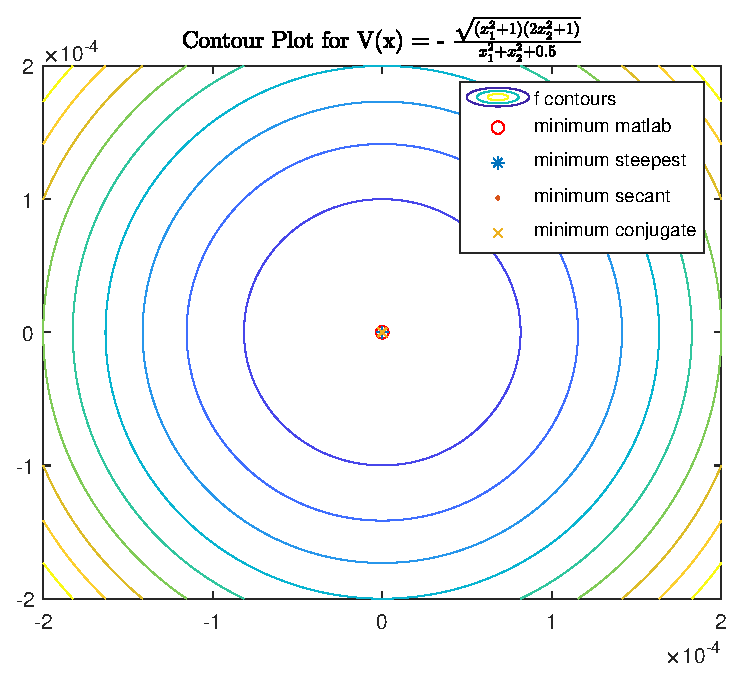
\includegraphics[width=0.4\textwidth]{images/matlab/matlab_1b.eps}
    \caption{Contour Plot for $V(x) = - \frac{\sqrt{(x_1^2 +1)(2x_2^2 + 1)}}{x_1^2 + x_2^2 + 0.5}$ }
\end{figure}